\documentclass[11pt]{article}
\usepackage[letterpaper,margin=0.65in]{geometry}
\usepackage[T1]{fontenc}
\usepackage[default]{sourcesanspro}
\usepackage{amsmath,amssymb,enumitem,fancyhdr,xcolor,tikz}
\usetikzlibrary{arrows.meta}
\setlength{\emergencystretch}{1em}
\setlength{\parindent}{0pt}\setlength{\parskip}{6pt}
\definecolor{ink}{HTML}{183642}
\pagestyle{fancy}\fancyhf{}\fancyhead[L]{\small\textcolor{ink}{Week 10 / Bridges / Adult return-visit guide}}
\fancyfoot[L]{\small Bellingham Math Circle / Week 10 / RV10-FAC-v1}\fancyfoot[R]{\small\thepage}
\renewcommand{\headrulewidth}{0.4pt}\renewcommand{\footrulewidth}{0pt}
\setlist[itemize]{leftmargin=1.2em,itemsep=2pt,topsep=2pt}
\newcommand{\parttitle}[1]{{\large\bfseries\color{ink}#1}\par}
\newcommand{\labelled}[2]{\textbf{#1} #2\par}
\begin{document}
\parttitle{Mathematical destination}
\labelled{One-way streets need balance.}{A finite directed town with at least one street has a closed walk using every street once iff each island has equally many incoming and outgoing streets and all islands with streets belong to one connected underlying town. Under the same connectivity condition, an open walk with different start and end exists iff one start has one more outgoing street, one end has one more incoming street, and all others balance. Ignore isolated islands. Arrows, not undirected degrees, govern this theorem. Multiple directed streets are allowed; a loop contributes one incoming and one outgoing street at its island.}
\labelled{Possible does not mean every choice works.}{Even a town with a complete bridge walk can strand a walker after a poor choice. In a triangle A--B--C--A with tail A--D, start at A and finish D. Taking A--D first isolates the token while three bridge counters remain. Avoid crossing a remaining bridge that disconnects the token from remaining work, unless it is the only available move. The destination counts even if it becomes isolated; merely counting remaining edge-bearing components misses this failure.}
\labelled{Overlaps save presses.}{A binary three-digit password can be covered in a linear sequence of ten button presses, and fewer cannot cover all eight passwords. A circular necklace of eight symbols also covers all eight windows, including those wrapping around the join. The directed overlap graph has islands 00, 01, 10, 11 and one street $abc$ from $ab$ to $bc$. Each island has two streets in and two out, so an Euler circuit gives a shortest necklace.}
\labelled{What children discover.}{Direction changes route feasibility; a local choice can consume a crucial bridge too soon; successive password windows can share symbols. Tests give examples. Incoming/outgoing counts explain impossibility, preserving access explains route choices, and a window-count lower bound plus a construction explains shortest length.}
\labelled{Band map.}{The first four arrow towns have a K--5 acted entry, with an adult reading labels; the four larger arrow towns and safe-choice pages suit grades 2--5. Grades 2--3 can compare failed/successful first choices and count arrows. Password pages are marked grades 4--5; a ready third grader who retains an ordered three-symbol window can join. Grades 4--5 can build the optional overlap graph and shortest-length proof. No graph terminology or formal notation is needed for entry. Independent older pages need no forced K--1 equivalent.}
\labelled{Status.}{Prepared, unpiloted; material fit and procedures not physically rehearsed. These turn the directed, Fleury and de Bruijn extension seeds named on base guide page 7 into usable investigations. The base student tasks develop undirected parity, repair and repeat counts. A return visit can develop one direction in depth.}
\newpage
\parttitle{Prepare and launch}
\labelled{Per pair.}{About 12 craft sticks, six blocks as islands, 16 bridge counters at most 0.75 inch across, one moving token at most 0.25 inch across (or a pencil tip for pointing), paper arrow slips, pencil and scrap paper. The printed towns use one-inch coordinate units; their active street-counter positions are spaced for these counters. Small arrow towns use 3.4-by-2.35-inch layout boxes and larger towns 6.8-by-3.2-inch boxes. These are layout boxes, not enclosing streets. Physical fit remains untested. For passwords prepare 24 separate button slips at most 0.5 inch wide: twelve marked 0 and twelve marked 1, or twelve counters of each of two colours no larger than 0.5 inch. Make an initial uncompressed 24-symbol row on the table; it would not fit a printed row. The 7.1-by-1.05-inch dashed row workspaces easily hold ten such buttons. Dashed 3.1-inch-diameter circles give active circle-construction space. Printed password cards and small convention diagrams are references. These fit calculations are digital, with no physical rehearsal. Use a three-hole paper frame, or a bracket drawn over three positions. Pencil rows need no slips. For an optional overlap graph, eight bridge counters remain separate from the button symbols. Counter size must fit the diagrams used physically; compact reference diagrams may instead be rebuilt with craft sticks on the table. Do not shrink an active town merely to fit more examples.}
\labelled{Visible rules.}{Put one counter on each street. Crossing picks up its counter, so used streets visibly close. In arrow towns the token follows the arrow. At a drawn crossing without an island, streets do not join. In safe-choice towns reset every counter before testing another route. In window tasks letters remain in place and the three-symbol frame slides one position at a time.}
\labelled{Launch together, 3--5 minutes.}{Let children arrange a small town, then show one legal arrow crossing and one rejected backward crossing. For the local-choice investigation, show how counters mark unused bridges without discussing the winning first choice. The printed arrow convention begins at X, crosses XY to Y and consumes that counter, then crosses YZ to Z and consumes the second. The ring shows the walker; dashed streets are used. Before password work use the printed non-task row 0110: its two-button window slides through 01,11,10. The circular example 011 keeps the buttons fixed and includes the joined last-first window 10. These input, intermediate and output visuals precede three-button tasks; they demonstrate conventions without solving the target construction.}
\labelled{First route and return.}{Pages 1--3 are arrow towns (page 1 K--5, pages 2--3 grades 2--5); pages 4--5 are grades 2--5 route choices; pages 6--7 are grades 4--5 passwords. Show the page 1 convention to all arrow walkers. Spend 15--25 minutes on two or three arrow towns or first-choice tests; later add a longer route or invent a town for a partner. A 20--30-minute return can start with physical password frames, then introduce the overlap graph only when it helps organise repeated windows. The upper trio can rotate mover, checker and recorder. Current staffing is three anchored adults for KK11 / 3333 / 445. Adults can read or scribe but should leave route and construction choices to children.}
\labelled{Records.}{One island word with visibly consumed counters is enough for a route. Password work needs one row plus its windows, derived afterward; no concurrent tally of presses and missing words is necessary. Record the exact town, arrows and rule, and note which further direction children want.}
\labelled{Source distinction.}{Lowell Fall 2025 \emph{Handout 10}, the second Problem 10.1, asked for shortest two-digit-password strings over three/four symbols. This is an acknowledged binary-triple/circular continuation with an explicit directed-route connection, not a claim of a new theme. Current Week 10 F10-v4 supplies undirected student Euler walks; its facilitator page 7 already names directed balance, Fleury and de Bruijn directions. The new companions instantiate those seeds with contrasting towns, active workspace, entry conventions and checked solutions; these directions are not claimed as absent from the collection. \emph{Math Circle by the Bay}, preface printed viii--x/PDF 9--11, supports manipulatives, varying depth and reserve problems; these exact tasks and preparation choices are our adaptations.}
\newpage
\parttitle{Problem 1 / Follow the arrows}
\labelled{Checking a town.}{For each island count arrows arriving and leaving. A closed all-street walk pairs every arrival with a departure. An open walk has an unpaired departure at its start and an unpaired arrival at its end; all intermediate visits still pair. Any different imbalance makes the requested walk impossible. Counts decide existence only when the underlying street-bearing town is connected.}
\labelled{Actual printed arrow towns.}{Town 1: A,B,C,A is a closed route, starting on any island by rotating that word. Town 2: impossible; outgoing-minus-incoming is $+2$ at A and $-2$ at C. Town 3: A,B,C,D, with unique start A and end D. Town 4: impossible; A,B,C,D have differences $+1,-2,+2,-1$. Town 5: A,B,C,D,A,C, start A and end C. Town 6: impossible; A,D,C have differences $+1,+2,-3$. Town 7: both cycles balance, but are disconnected; no single route covers them. Town 8: A,B,C,A,D,E,A is a closed route; any island can start a rotation. Each word crosses exactly the drawn streets in their arrow directions.}
\labelled{Why balance is sufficient.}{In a finite balanced connected directed town, begin on an island with a street and follow unused outgoing streets. You cannot get stuck at a different island: there, an extra arrival would imply an unused departure. Thus you close a directed loop. If unused streets remain, connectivity provides a visited island with unused outgoing work; make another loop there and splice it into the route. Repeat until every street is used.}
\labelled{Open walks.}{If exactly one start has outgoing-minus-incoming equal to 1 and exactly one end has incoming-minus-outgoing equal to 1, temporarily add a street from end to start. The augmented town balances and has a closed all-street walk. Cut that walk at the added street and omit it, giving a walk from the required start to end. This is an adult explanation; children can discover the unmatched departure and arrival with counters.}
\labelled{Arrow changes can matter.}{An undirected triangle is always one-stroke, but orienting its streets A to B, A to C and B to C, as in Town 2, creates incompatible differences. Conversely, directing a cycle consistently balances every island. The ordinary odd-island criterion alone cannot decide a directed town. Always inspect the actual arrows rather than the outline.}
\labelled{Hint and continuation.}{If a child is stuck, lay arrivals and departures as two piles beside one island and pair them. Later ask them to orient a familiar undirected town so a closed route works, or create an open arrow town with chosen start and finish. Retain the child's arrow choices as mathematical work, not merely another diagram of the base degree rule.}
\labelled{Limit.}{These statements concern finite streets, each used exactly once, and ordinary connected underlying towns. They do not assert a route through disconnected groups, or a route obeying additional turn restrictions. If the diagram has two directions on one physical road, treat them as two distinct streets with two counters.}
\newpage
\parttitle{Problem 2 / A route can paint itself into a corner}
\labelled{The smallest checked trap.}{For triangle edges AB,BC,CA and tail AD, the odd islands are A and D. From A a complete route is A,B,C,A,D, or its reverse-triangle alternative A,C,B,A,D. Starting with AD leaves the token at D with the triangle untouched and no available departure. Starting at D forces DA first, then either triangle direction works.}
\labelled{All four printed start tests.}{Town 1 (star A): AB and AC allow completion; AD strands the walker. Town 2 (star D): DA is the only first street and is safe; D,A,B,C,A completes it. Town 3 (star A, square with diagonal AC): all AB,AD,AC are safe; completions are A,B,C,D,A,C; A,D,C,B,A,C; and A,C,B,A,D,C. Town 4 (star A, two triangles joined by AD): AB and AC are safe, AD is unsafe. Complete the left triangle, then cross AD once and complete the right triangle, for example A,B,C,A,D,E,F,D. The starting stars and resets are part of the experiment.}
\labelled{Safe local test.}{After tentatively choosing a bridge, ask whether the new token location can still reach every remaining bridge without using the chosen one again. Include the new location even when it has no remaining incident bridge. If remaining work is unreachable and another choice was available, undo this attempt and try another bridge. This is a reasoning prompt for adults to offer after failures, not a required printed algorithm.}
\labelled{Why this preserves a complete walk.}{After a legal step from a feasible Euler state, the remaining degrees still have the correct odd endpoints, with the token as the next start. If every remaining edge is reachable from that token, Euler's theorem gives a completion. Losing reachability is therefore exactly the obstruction created by a bad choice. In the usual Fleury formulation, avoid a bridge of the remaining graph when another incident edge is available; take a bridge when it is forced. The graph includes its current and destination vertices.}
\labelled{An elementary view.}{A bridge is the only connection between two parts. Crossing it uses that connection forever. If you leave unused counters behind in the old part, they can no longer be collected. Finish that part before crossing, unless nothing remains there. On a closed all-even town there is no bridge: summing the degrees of either side of one would give an odd total, contradicting all even degrees.}
\labelled{Questions and hint.}{Compare two first moves in a town already known to be possible. Ask which counters become unreachable after one choice and why resetting makes another route possible. If needed, physically separate the two parts after removing the crucial craft stick. Keep the failed route: it is useful evidence, not a mistake to erase.}
\labelled{Continuation.}{On Town 4 compare crossing AD first with crossing it after finishing the left triangle. Later pause a legal route partway and test which next choices still permit completion. Invent a town where only some first choices work. A rule that preserves access does not demand the globally fewest repeats, another question already developed in base Week 10. Save successful and failed island words with their starting islands.}
\newpage
\parttitle{Problem 3 / Passwords that overlap}
\labelled{Shortest linear construction.}{The ten-symbol string 0001011100 has successive three-symbol windows 000, 001, 010, 101, 011, 111, 110, 100. Those are all eight binary triples exactly once. Any linear string of length $L$ has at most $L-2$ triple windows, so fewer than ten symbols cannot cover eight different passwords. A construction reaching the lower bound proves optimality.}
\labelled{Shortest circular construction.}{The necklace 00010111 has the same eight windows, with 110 and 100 wrapping across its join. Eight positions provide only eight length-three windows, so fewer than eight positions cannot cover all passwords. Rotating the necklace gives the same circular arrangement unless a starting point is deliberately marked. Reversing or swapping colours can be declared equivalent only if the task says so.}
\labelled{A non-task window-to-street bridge.}{ABC becomes a street from AB to BC; BCD becomes a street from BC to CD. The first two and last two letters name its islands. The shared BC joins the streets. Begin with AB, then append C and D to recover ABCD. Show this conversion only when the children choose to use the optional map.}
\begin{center}
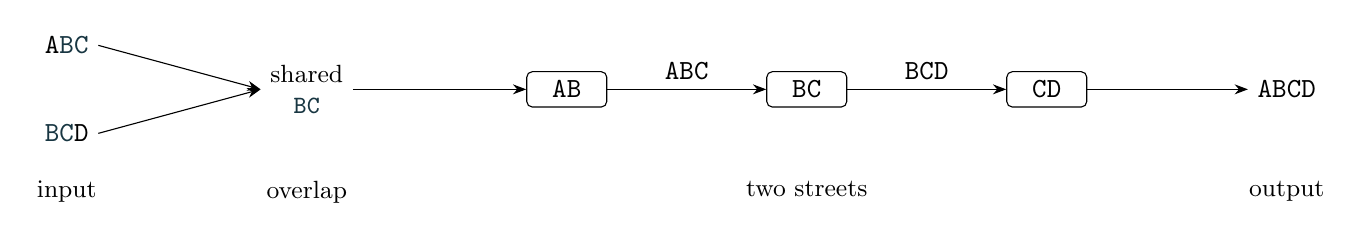
\begin{tikzpicture}[x=1in,y=1in,>=Stealth,font=\small]
\node[font=\ttfamily] (first) at (.25,.66) {A\textcolor{ink}{BC}};
\node[font=\ttfamily] (second) at (.25,.22) {\textcolor{ink}{BC}D};
\node[align=center] (shared) at (1.45,.44) {shared\\\textcolor{ink}{\ttfamily BC}};
\draw[->] (first.east)--(shared.west);
\draw[->] (second.east)--(shared.west);
\node[draw,rounded corners=2pt,font=\ttfamily,minimum width=.4in] (ab) at (2.75,.44) {AB};
\node[draw,rounded corners=2pt,font=\ttfamily,minimum width=.4in] (bc) at (3.95,.44) {BC};
\node[draw,rounded corners=2pt,font=\ttfamily,minimum width=.4in] (cd) at (5.15,.44) {CD};
\draw[->] (shared.east)--(ab.west);
\draw[->] (ab)--node[above,font=\ttfamily]{ABC}(bc);
\draw[->] (bc)--node[above,font=\ttfamily]{BCD}(cd);
\node[font=\ttfamily] (word) at (6.35,.44) {ABCD};
\draw[->] (cd.east)--(word.west);
\node[anchor=north] at (.25,.03) {input};
\node[anchor=north] at (1.45,.03) {overlap};
\node[anchor=north] at (3.95,.03) {two streets};
\node[anchor=north] at (6.35,.03) {output};
\end{tikzpicture}
\end{center}
\labelled{From windows to streets.}{A triple $abc$ shares its last two symbols $bc$ with the next window's first two. Represent it by a directed street from $ab$ to $bc$. On islands 00, 01, 10, 11 each island has two incoming and two outgoing streets, including loops 000 and 111. The graph is connected, hence Eulerian. One circuit uses street labels in order 000, 001, 010, 101, 011, 111, 110, 100. Write its initial 00, then append the final symbol of each street; this yields the ten-symbol linear string. Close the circle and discard the repeated final two symbols to obtain the necklace.}
\labelled{Physical entry and hint.}{Use counters and a three-hole frame to check a proposed row. Repeated windows waste potential coverage; windows that share two symbols can follow without starting again. If a child needs a hint, put two selected triples together and ask which counters can be shared. Introduce the four-island map only after that overlap is meaningful.}
\labelled{Continuation.}{There are two binary triple necklaces up to rotation: 00010111 and 00011101. This optional finite fact is checked by enumerating all 256 eight-symbol rows and identifying rotations, not assumed from the construction. Larger alphabets or longer windows give further visits; the graph then has length-$(n-1)$ words as vertices and length-$n$ words as streets. Formal graph counting is optional.}
\labelled{Record.}{Preserve the final row/necklace and the window list that checks it. Mark whether the child found an example, established the lower bound, or made the overlap-street connection. The prior-year two-digit password question is related history, not counted as another new investigation.}

\end{document}
